% !TeX spellcheck = en_US
%\documentclass[11pt,a4paper]{article}
\documentclass[11pt
  , a4paper
  , article
  , oneside
%  , twoside
%  , draft
]{memoir}

\usepackage{control}
\usepackage[numbers]{natbib}


\begin{document}

\newcommand{\technumber}{
  RAON Control-Document Series\\
  Revision : v1.0,   Release : 2015-03-16 fixed date}
\title{\textbf{FPGA - Zynq}}

\author{이상일\thanks{silee7103@ibs.re.kr}, 손창욱 \\

  Rare Isotope Science Project\\
  Institute for Basic Science, Daejeon, South Korea
}
\date{\today}

\renewcommand{\maketitlehooka}{\begin{flushright}\textsf{\technumber}\end{flushright}}
%\renewcommand{\maketitlehookb}{\centering\textsf{\subtitle}}
%\renewcommand{\maketitlehookc}{C}
%\renewcommand{\maketitlehookd}{D}

\maketitle

\begin{abstract}
RAON is a particle accelerator to research the interaction between the nucleus forming a rare isotope as Korean heavy-ion accelerator. RAON accelerator consists of a number of facilities and equipments as a large-scaled experimental device operating under the distributed environment. For synchronization control between these experimental devices, timing system of the RAON uses the VME-based EVG/EVR system. This paper is intended to test high-speed device control with timing event signal. To test the high-speed performance of the control logic with the minimized event signal delay, we are planing to establish the step motor controller testbed applying the FPGA chip. The testbed controller will be configured with Zynq 7000 series of Xilinx FPGA chip. Zynq as SoC (System on Chip) is divided into PS (Processing System) with PL (Programmable Logic). PS with the dual-core ARM cpu is performing the high-level control logic at run-time on linux operating system. PL with the low-level FPGA I/O signal interfaces with the step motor controller directly with the event signal received from timing system.

This paper describes the content and performance evaluation obtaining from the step motor control through the various synchronized event signal received from the timing system.

\end{abstract}

\clearpage

FPGA(Field Programmable Gate Array)는 Hardware의 IC 소자의 gate array를 사용자가 program하여 회로를 구성할 수 있는 chip을 말한다. FPGA 프로그램 개발은 HDL(Hardware Description Language) 개발표준 언어를 사용하며 프로그램 할 수 있으며 아래와 같은 두 가지 HDL 언어를 지원한다.

\begin{itemize}
	\item VHDL
	\item Verilog HDL
\end{itemize}

본 문서에는 Xilinx의 FPGA Chip 중 Zynq 사용을 위한 내용을 기술한다. Zynq의 특징은 앞서 설명한 FPGA의 특징과 ARM CPU를 내장한 embedded 특징 모두 가지는 하나의 SoC(System on Chip) 이다.  따라서 Zynq Chip에는 기존 FPGA에 가지는 장점에 embedded 형태의 운영체제를 가질 수 있는 장점이 있다. 또한 이 둘간의 interface는 AXI Bus interface를 통한 메모리 맵을 통하여 데이터 통신이 가능하다. 따라서 고속 신호처리를 위하여는 FPGA I/O를 low level(hardware) 단에서 처리를 하며, 상위 레벨과의 인터페이스 및 주요 제어로직은 CPU 모듈에서 처리 할 수 있는 설계가 가능하다. 이는 가속기 제어 operation sequence에 따른 timing event의 external trigger를 입력으로 받아 고속의 신호를 처리하여야 하는 application에 활용 할 수 있다. 또한 MPS(Machine Protection System)와 같은 고속의 application에 적용할 수 있으리라 판단된다.
Zynq는 ARM 계열의 CPU를 가지고 있으며 여기에 linux 운영체제를 쉽게 올릴 수 있는 petalinux softeware tool을 제공한다. 

\begin{figure}[h!]
	\centering
	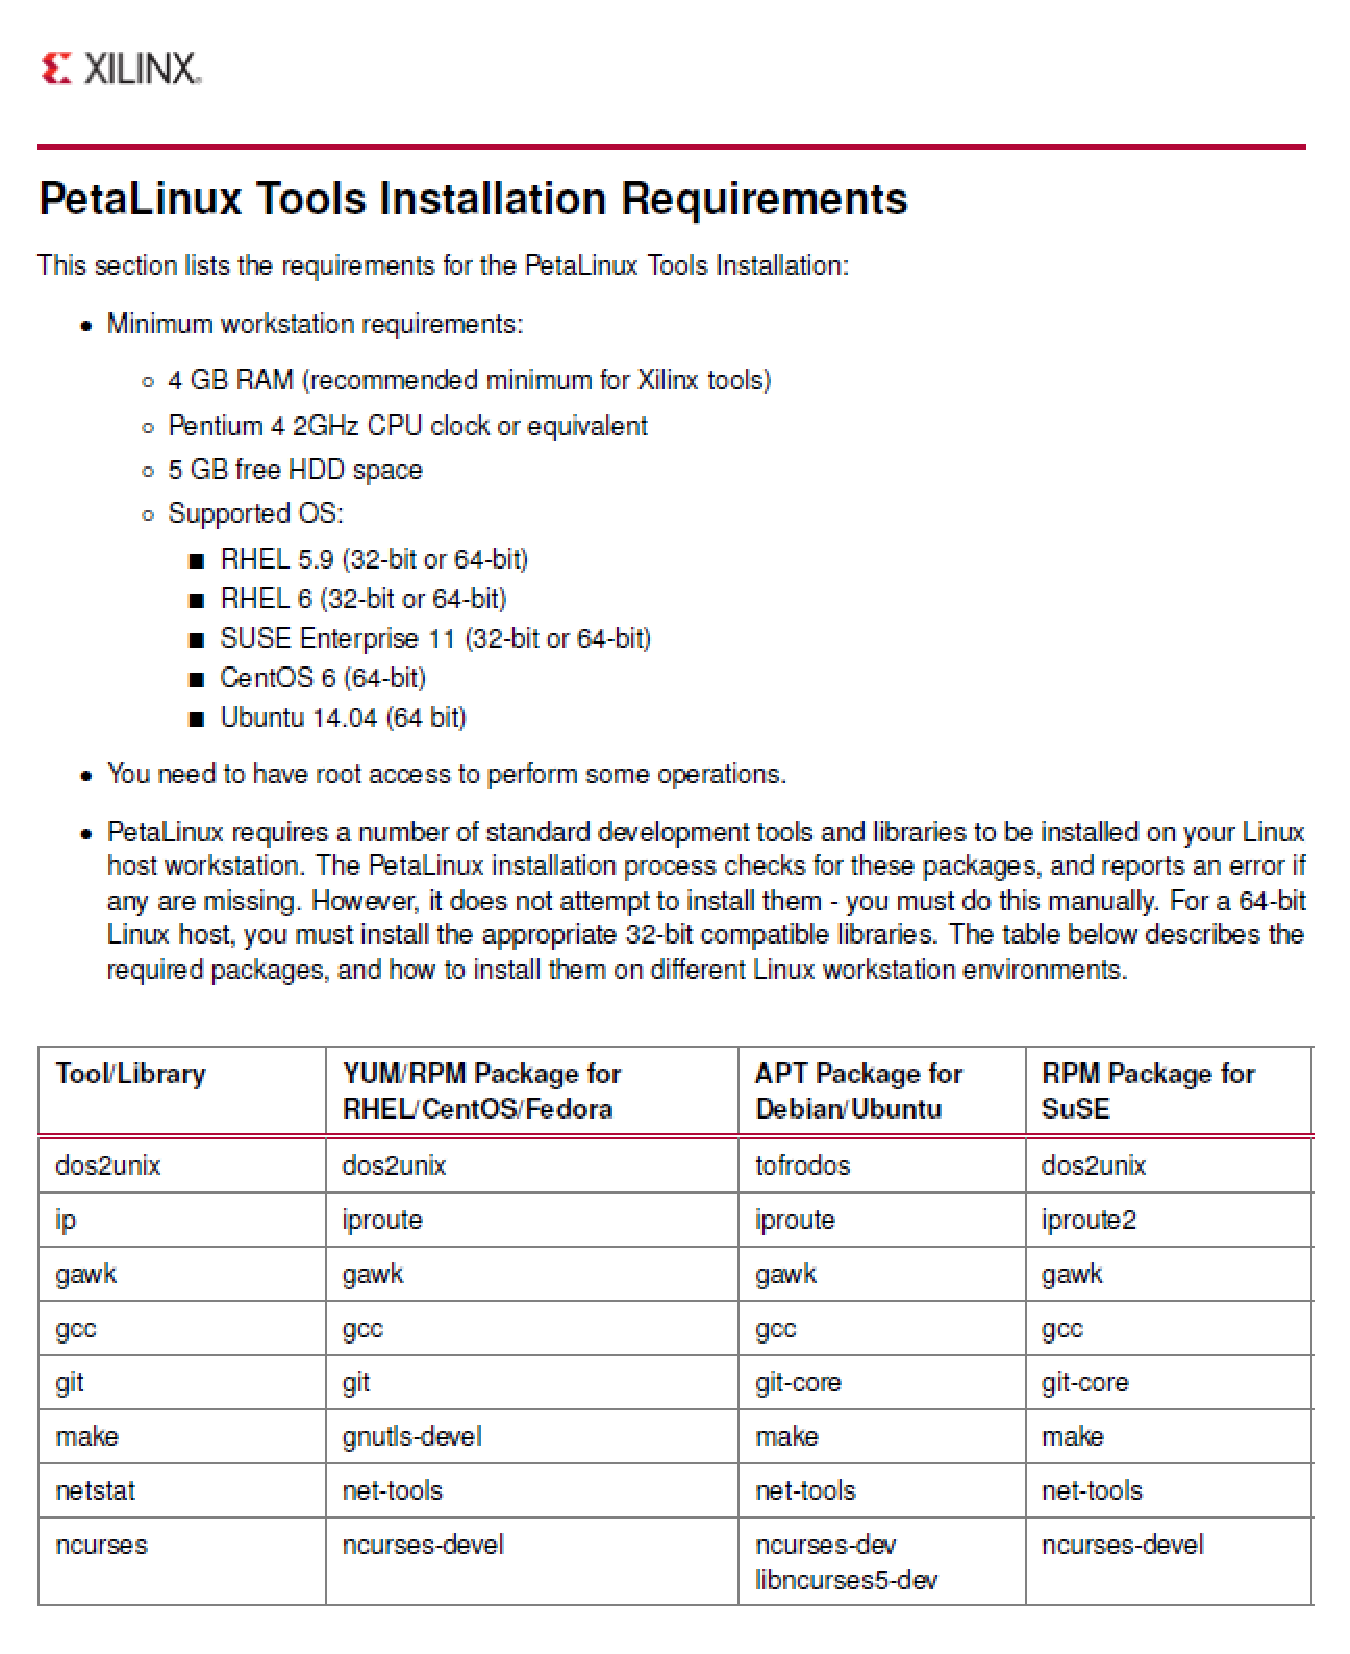
\includegraphics[width=0.85\textwidth]{./images/preinstall_2.eps}
	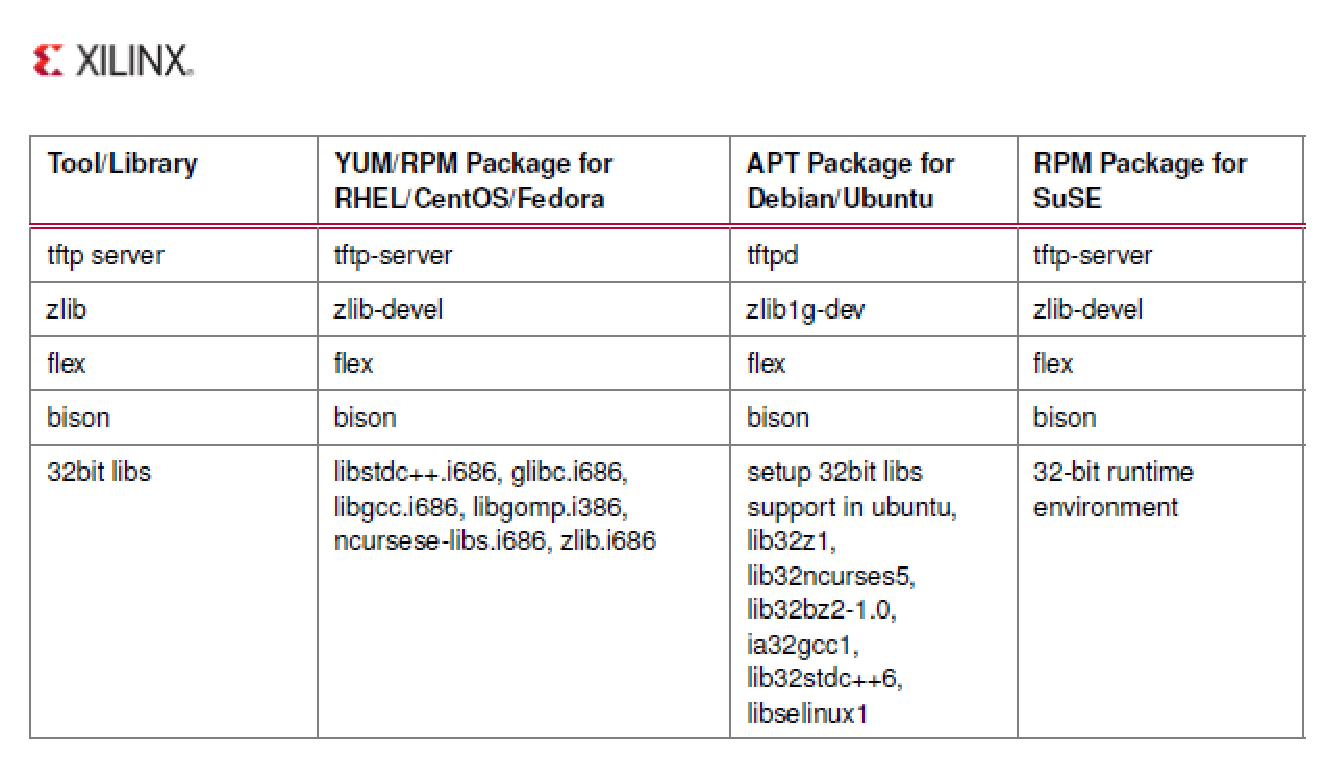
\includegraphics[width=0.85\textwidth]{./images/preinstall_3.eps}
	\caption{Pre-install packcages}
	\label{fig:preinstall_2} 
\end{figure}

\clearpage


Xilinx에서 제공하는 linux image를 생성하는 툴인 peta-linux를 설치하기 위하여 그림 \ref{fig:preinstall_2} 에서와 같이 Debian/Ubuntu에서 언급한 내용을 설치한다. 이는 64bit 환경하에서 petalinux를 설치하기 위한 추가적 32bit용 패키지 모듈이다.

아래 리스트는 상위 그림 \ref{fig:preinstall_2} 에서 언급한 모듈에 대한 설치 내용을 보여준다.


\begin{lstlisting}[style=termstyle]
root@silee:/home/ctrluser# cat typescript 
Script started on Tue 07 Apr 2015 10:23:32 AM KST
root@silee:/home/ctrluser# 
root@silee:/home/ctrluser# aptitude install tofrodos
The following NEW packages will be installed:
tofrodos 
0 packages upgraded, 1 newly installed, 0 to remove and 0 not upgraded.
Need to get 21.9 kB of archives. After unpacking 68.6 kB will be used.
Get: 1 http://ftp.debian.org/debian/ wheezy/main tofrodos amd64 1.7.9.debian.1-1 [21.9 kB]
Fetched 21.9 kB in 2s (8,759 B/s)   
Selecting previously unselected package tofrodos.
(Reading database ... 317356 files and directories currently installed.)
Unpacking tofrodos (from .../tofrodos_1.7.9.debian.1-1_amd64.deb) ...
Processing triggers for man-db ...
Setting up tofrodos (1.7.9.debian.1-1) ...

root@silee:/home/ctrluser# aptitude install iproute gawk git-core
The following NEW packages will be installed:
gawk git-core 
0 packages upgraded, 2 newly installed, 0 to remove and 0 not upgraded.
Need to get 973 kB of archives. After unpacking 2,345 kB will be used.
Get: 1 http://ftp.debian.org/debian/ wheezy/main gawk amd64 1:4.0.1+dfsg-2.1 [972 kB]
Get: 2 http://ftp.debian.org/debian/ wheezy/main git-core all 1:1.7.10.4-1+wheezy1 [1,336B]
Fetched 973 kB in 8s (116 kB/s)
Selecting previously unselected package gawk.
(Reading database ... 317366 files and directories currently installed.)
Unpacking gawk (from .../gawk_1%3a4.0.1+dfsg-2.1_amd64.deb) ...
Selecting previously unselected package git-core.
Unpacking git-core (from .../git-core_1%3a1.7.10.4-1+wheezy1_all.deb) ...
Processing triggers for man-db ...
Setting up gawk (1:4.0.1+dfsg-2.1) ...
Setting up git-core (1:1.7.10.4-1+wheezy1) ...

root@silee:/home/ctrluser# aptitude install net-tools
No packages will be installed, upgraded, or removed.
0 packages upgraded, 0 newly installed, 0 to remove and 0 not upgraded.
Need to get 0 B of archives. After unpacking 0 B will be used.

root@silee:/home/ctrluser# aptitude search net-tools
i   net-tools                - The NET-3 networking toolkit                                       
root@silee:/home/ctrluser# aptitude search ncurses-dev
p   libcunit1-ncurses-dev                   - Unit Testing Library for C (ncurses) -- development files          
p   libghc-ncurses-dev                      - Haskell bindings to the GNU ncurses library                        
v   libghc-ncurses-dev-0.2.1-8df37    		-                                                                    
p   libkaya-ncurses-dev                     - Ncurses binding for kaya                                           
v   libncurses-dev    						-      
v   ncurses-dev       						-
                                                                    
root@silee:/home/ctrluser# aptitude install ncurses-dev
Note: selecting "libncurses5-dev" instead of the
virtual package "ncurses-dev"
The following NEW packages will be installed:
libncurses5-dev 
0 packages upgraded, 1 newly installed, 0 to remove and 0 not upgraded.
Need to get 223 kB of archives. After unpacking 1,032 kB will be used.
Get: 1 http://ftp.debian.org/debian/ wheezy/main libncurses5-dev amd64 5.9-10 [223 kB]
Fetched 223 kB in 3s (59.8 kB/s)          
Selecting previously unselected package libncurses5-dev.
(Reading database ... 317477 files and directories currently installed.)
Unpacking libncurses5-dev (from .../libncurses5-dev_5.9-10_amd64.deb) ...
Setting up libncurses5-dev (5.9-10) ...

root@silee:/home/ctrluser# aptitude search ncurses-dev
p   libcunit1-ncurses-dev                    - Unit Testing Library for C (ncurses) -- development files          
p   libghc-ncurses-dev                       - Haskell bindings to the GNU ncurses library                        
v   libghc-ncurses-dev-0.2.1-8df37           -                                                                    
p   libkaya-ncurses-dev                      - Ncurses binding for kaya                                           
v   libncurses-dev   						 -                                                                    
v   ncurses-dev                              -                                                                 
   
root@silee:/home/ctrluser# aptitude search libncurses5-dev
i   libncurses5-dev                          - developer's libraries for ncurses                                  
root@silee:/home/ctrluser# aptitude install tftpd
The following NEW packages will be installed:
openbsd-inetd{a} tftpd 
0 packages upgraded, 2 newly installed, 0 to remove and 0 not upgraded.
Need to get 55.1 kB of archives. After unpacking 109 kB will be used.
Do you want to continue? [Y/n/?] Y
Get: 1 http://ftp.debian.org/debian/ wheezy/main openbsd-inetd amd64 0.20091229-2 [38.1 kB]
Get: 2 http://ftp.debian.org/debian/ wheezy/main tftpd amd64 0.17-18 [17.0 kB]
Fetched 55.1 kB in 2s (23.4 kB/s)  
Selecting previously unselected package openbsd-inetd.
(Reading database ... 317514 files and directories currently installed.)
Unpacking openbsd-inetd (from .../openbsd-inetd_0.20091229-2_amd64.deb) ...
Selecting previously unselected package tftpd.
Unpacking tftpd (from .../tftpd_0.17-18_amd64.deb) ...
Processing triggers for man-db ...
Setting up openbsd-inetd (0.20091229-2) ...
[ ok ] Stopping internet superserver: inetd.
[info] Not starting internet superserver: no services enabled.
Setting up tftpd (0.17-18) ...

root@silee:/home/ctrluser# aptitude install zlib1g-dev
No packages will be installed, upgraded, or removed.
0 packages upgraded, 0 newly installed, 0 to remove and 0 not upgraded.
Need to get 0 B of archives. After unpacking 0 B will be used.

root@silee:/home/ctrluser# aptitude search zlib1g
i   zlib1g                              - compression library - runtime                                      
p   zlib1g-dbg                          - compression library - development                                  
i A zlib1g-dev                          - compression library - development                                  
root@silee:/home/ctrluser# aptitude search flex
p   cl-flexi-streams                    - Flexi-streams: Flexible bivalent streams for Common Lisp           
p   cl-flexichain                       - An efficient gap buffer with a well-defined external protocol      
p   flex                                - A fast lexical analyzer generator.                                 
p   flex-doc                            - Documentation for flex (a fast lexical analyzer generator).        
p   flex-old                            - Old version of the fast lexical analyzer generator                 
p   flex-old-doc                        - Documentation for an old flex (a fast lexical analyzer generator)  
p   flexbackup                          - Flexible backup tool for small to medium sized installations       
p   flexc++                             - Flex-style scanner generator for C++                               
p   flexloader                          - utility to configure SRAM based ALTERA devices                     
v   flexmem                             -                                                                    
p   flexml                              - Fast validating XML processors and applications generator          
p   jflex                               - lexical analyzer generator for Java                                
p   libdatetime-format-flexible-perl    - Perl module to transform strings into DateTime objects             
p   libflexdock-java                    - Swing Java docking framework                                       
p   libflexdock-java-demo               - Swing Java docking framework - demos and examples                  
p   libflexdock-java-doc                - Swing Java docking framework - demos and examples                  
p   libflexmock-ruby                    - Transitional package for ruby-flexmock                             
p   libflexmock-ruby1.8                 - Transitional package for ruby-flexmock                             
p   libflexmock-ruby1.9.1               - Transitional package for ruby-flexmock                             
p   python-flexmock                     - Mock/Stub/Spy library for Python                                   
p   python3-flexmock                    - Mock/Stub/Spy library for Python 3                                 
p   ruby-flexmock                       - simple and flexible mock objects for testing                       
root@silee:/home/ctrluser# aptitude search flex
p   cl-flexi-streams                    - Flexi-streams: Flexible bivalent streams for Common Lisp           
p   cl-flexichain                       - An efficient gap buffer with a well-defined external protocol      
p   flex                                - A fast lexical analyzer generator.                                 
p   flex-doc                            - Documentation for flex (a fast lexical analyzer generator).        
p   flex-old                            - Old version of the fast lexical analyzer generator                 
p   flex-old-doc                        - Documentation for an old flex (a fast lexical analyzer generator)  
p   flexbackup                          - Flexible backup tool for small to medium sized installations       
p   flexc++                             - Flex-style scanner generator for C++                               
p   flexloader                          - utility to configure SRAM based ALTERA devices                     
v   flexmem                             -                                                                    
p   flexml                              - Fast validating XML processors and applications generator          
p   jflex                               - lexical analyzer generator for Java                                
p   libdatetime-format-flexible-perl    - Perl module to transform strings into DateTime objects             
p   libflexdock-java                    - Swing Java docking framework                                       
p   libflexdock-java-demo               - Swing Java docking framework - demos and examples                  
p   libflexdock-java-doc                - Swing Java docking framework - demos and examples                  
p   libflexmock-ruby                    - Transitional package for ruby-flexmock                             
p   libflexmock-ruby1.8                 - Transitional package for ruby-flexmock                             
p   libflexmock-ruby1.9.1               - Transitional package for ruby-flexmock                             
p   python-flexmock                     - Mock/Stub/Spy library for Python                                   
p   python3-flexmock                    - Mock/Stub/Spy library for Python 3                                 
p   ruby-flexmock                       - simple and flexible mock objects for testing                       
root@silee:/home/ctrluser# aptitude install flex
The following NEW packages will be installed: flex 
0 packages upgraded, 1 newly installed, 0 to remove and 0 not upgraded.
Need to get 332 kB of archives. After unpacking 944 kB will be used.
Get: 1 http://ftp.debian.org/debian/ wheezy/main flex amd64 2.5.35-10.1 [332 kB]
Fetched 332 kB in 4s (71.4 kB/s)
Selecting previously unselected package flex.
(Reading database ... 317530 files and directories currently installed.)
Unpacking flex (from .../flex_2.5.35-10.1_amd64.deb) ...
Processing triggers for install-info ...
Processing triggers for man-db ...
Setting up flex (2.5.35-10.1) ...

root@silee:/home/ctrluser# aptitude install bison
The following NEW packages will be installed:
bison libbison-dev{a} 
0 packages upgraded, 2 newly installed, 0 to remove and 0 not upgraded.
Need to get 977 kB of archives. After unpacking 1,846 kB will be used.
Do you want to continue? [Y/n/?] Y
Get: 1 http://ftp.debian.org/debian/ wheezy/main libbison-dev amd64 1:2.5.dfsg-2.1 [289 kB]
Get: 2 http://ftp.debian.org/debian/ wheezy/main bison amd64 1:2.5.dfsg-2.1 [689 kB]
Fetched 977 kB in 7s (126 kB/s)                                                                                                    
Selecting previously unselected package libbison-dev:amd64.
(Reading database ... 317569 files and directories currently installed.)
Unpacking libbison-dev:amd64 (from .../libbison-dev_1%3a2.5.dfsg-2.1_amd64.deb) ...
Selecting previously unselected package bison.
Unpacking bison (from .../bison_1%3a2.5.dfsg-2.1_amd64.deb) ...
Processing triggers for man-db ...
Setting up libbison-dev:amd64 (1:2.5.dfsg-2.1) ...
Setting up bison (1:2.5.dfsg-2.1) ...
update-alternatives: using /usr/bin/bison.yacc to provide /usr/bin/yacc (yacc) in auto mode

root@silee:/home/ctrluser# aptitude search lib32z1
p   lib32z1                                   - compression library - 32 bit runtime                               
p   lib32z1-dev                               - compression library - 32 bit development                           

root@silee:/home/ctrluser# aptitude install lib32z1
The following NEW packages will be installed:
lib32z1 libc6-i386{a} 
0 packages upgraded, 2 newly installed, 0 to remove and 0 not upgraded.
Need to get 4,111 kB of archives. After unpacking 9,407 kB will be used.
Do you want to continue? [Y/n/?] Y
Get: 1 http://security.debian.org/ wheezy/updates/main libc6-i386 amd64 2.13-38+deb7u8 [4,022 kB]
Get: 2 http://ftp.debian.org/debian/ wheezy/main lib32z1 amd64 1:1.2.7.dfsg-13 [89.0 kB]
Fetched 4,111 kB in 2s (1,444 kB/s)                                    
Selecting previously unselected package libc6-i386.
(Reading database ... 317676 files and directories currently installed.)
Unpacking libc6-i386 (from .../libc6-i386_2.13-38+deb7u8_amd64.deb) ...
Selecting previously unselected package lib32z1.
Unpacking lib32z1 (from .../lib32z1_1%3a1.2.7.dfsg-13_amd64.deb) ...
Setting up libc6-i386 (2.13-38+deb7u8) ...
Setting up lib32z1 (1:1.2.7.dfsg-13) ...

root@silee:/home/ctrluser# aptitude search lib32z1
i   lib32z1                                   - compression library - 32 bit runtime                               
p   lib32z1-dev                               - compression library - 32 bit development                           
root@silee:/home/ctrluser# aptitude search lib32ncurses5
p   lib32ncurses5                             - shared libraries for terminal handling (32-bit)                    
p   lib32ncurses5-dev                         - developer's libraries for ncurses (32-bit)                         
root@silee:/home/ctrluser# aptitude install lib32ncurses5
The following NEW packages will be installed:
lib32ncurses5 lib32tinfo5{a} 
0 packages upgraded, 2 newly installed, 0 to remove and 0 not upgraded.
Need to get 384 kB of archives. After unpacking 688 kB will be used.
Do you want to continue? [Y/n/?] Y
Get: 1 http://ftp.debian.org/debian/ wheezy/main lib32tinfo5 amd64 5.9-10 [268 kB]
Get: 2 http://ftp.debian.org/debian/ wheezy/main lib32ncurses5 amd64 5.9-10 [115 kB]
Fetched 384 kB in 5s (74.4 kB/s)        
Selecting previously unselected package lib32tinfo5.
(Reading database ... 317986 files and directories currently installed.)
Unpacking lib32tinfo5 (from .../lib32tinfo5_5.9-10_amd64.deb) ...
Selecting previously unselected package lib32ncurses5.
Unpacking lib32ncurses5 (from .../lib32ncurses5_5.9-10_amd64.deb) ...
Setting up lib32tinfo5 (5.9-10) ...
Setting up lib32ncurses5 (5.9-10) ...

root@silee:/home/ctrluser# aptitude install lib32bz2
Couldn't find package "lib32bz2".  However, the following
packages contain "lib32bz2" in their name:
lib32bz2-1.0 lib32bz2-dev 
Couldn't find package "lib32bz2".  However, the following
packages contain "lib32bz2" in their name:
lib32bz2-1.0 lib32bz2-dev 
No packages will be installed, upgraded, or removed.
0 packages upgraded, 0 newly installed, 0 to remove and 0 not upgraded.
Need to get 0 B of archives. After unpacking 0 B will be used.

root@silee:/home/ctrluser# aptitude search lib32bz2
p   lib32bz2-1.0                              - high-quality block-sorting file compressor library - 32bit runtime 
p   lib32bz2-dev                              - high-quality block-sorting file compressor library - 32bit developm
root@silee:/home/ctrluser# aptitude install lib32bz2-1.0
The following NEW packages will be installed: lib32bz2-1.0 
0 packages upgraded, 1 newly installed, 0 to remove and 0 not upgraded.
Need to get 40.5 kB of archives. After unpacking 77.8 kB will be used.
Get: 1 http://ftp.debian.org/debian/ wheezy/main lib32bz2-1.0 amd64 1.0.6-4 [40.5 kB]
Fetched 40.5 kB in 1s (21.3 kB/s)       
Selecting previously unselected package lib32bz2-1.0.
(Reading database ... 318003 files and directories currently installed.)
Unpacking lib32bz2-1.0 (from .../lib32bz2-1.0_1.0.6-4_amd64.deb) ...
Setting up lib32bz2-1.0 (1.0.6-4) ...

root@silee:/home/ctrluser# aptitude search lib32gcc
p   lib32gcc1                                 - GCC support library (32 bit Version)                               
p   lib32gcc1-dbg                             - GCC support library (debug symbols)                                
root@silee:/home/ctrluser# aptitude search lib32stdc++
p   lib32stdc++6                              - GNU Standard C++ Library v3 (32 bit Version)                       
p   lib32stdc++6-4.4-dbg                      - GNU Standard C++ Library v3 (debugging files)                      
p   lib32stdc++6-4.6-dbg                      - GNU Standard C++ Library v3 (debugging files)                      
p   lib32stdc++6-4.7-dbg                      - GNU Standard C++ Library v3 (debugging files)                      
root@silee:/home/ctrluser# aptitude install lib32stdc++6
The following NEW packages will be installed:
lib32gcc1{a} lib32stdc++6 
0 packages upgraded, 2 newly installed, 0 to remove and 0 not upgraded.
Need to get 400 kB of archives. After unpacking 1,336 kB will be used.
Do you want to continue? [Y/n/?] Y
Get: 1 http://ftp.debian.org/debian/ wheezy/main lib32gcc1 amd64 1:4.7.2-5 [53.2 kB]
Get: 2 http://ftp.debian.org/debian/ wheezy/main lib32stdc++6 amd64 4.7.2-5 [346 kB]
Fetched 400 kB in 5s (70.3 kB/s)       
Selecting previously unselected package lib32gcc1.
(Reading database ... 318009 files and directories currently installed.)
Unpacking lib32gcc1 (from .../lib32gcc1_1%3a4.7.2-5_amd64.deb) ...
Selecting previously unselected package lib32stdc++6.
Unpacking lib32stdc++6 (from .../lib32stdc++6_4.7.2-5_amd64.deb) ...
Setting up lib32gcc1 (1:4.7.2-5) ...
Setting up lib32stdc++6 (4.7.2-5) ...

root@silee:/home/ctrluser# aptitude search libselinux1
i   libselinux1                               - SELinux runtime shared libraries                                   
p   libselinux1-dev                           - SELinux development headers                                        
root@silee:/home/ctrluser# aptitude search libgtk2.0
i A libgtk2.0-0                               - GTK+ graphical user interface library                              
p   libgtk2.0-0-dbg                           - GTK+ libraries and debugging symbols                               
i A libgtk2.0-bin                             - programs for the GTK+ graphical user interface library             
i A libgtk2.0-cil                             - CLI binding for the GTK+ toolkit 2.12                              
p   libgtk2.0-cil-dev                         - CLI binding for the GTK+ toolkit 2.12                              
i A libgtk2.0-common                          - common files for the GTK+ graphical user interface library         
p   libgtk2.0-dev                             - development files for the GTK+ library                             
p   libgtk2.0-doc                             - documentation for the GTK+ graphical user interface library        
root@silee:/home/ctrluser# aptitude search libgtk2.0:i386
root@silee:/home/ctrluser# aptitude search libgtk2.0-0
i A libgtk2.0-0                               - GTK+ graphical user interface library                              
p   libgtk2.0-0-dbg                           - GTK+ libraries and debugging symbols                               
root@silee:/home/ctrluser# aptitude search libgtk2.0-0:i386
root@silee:/home/ctrluser# aptitude search libncurse
v   libncurses-dev                            -                                                                    
p   libncurses-gst                            - Ncurses bindings for GNU Smalltalk                                 
p   libncurses-ruby                           - Transitional package for ruby-ncurses                              
p   libncurses-ruby1.8                        - Transitional package for ruby-ncurses                              
p   libncurses-ruby1.9                        - Transitional package for ruby-ncurses                              
p   libncurses-ruby1.9.1                      - Transitional package for ruby-ncurses                              
i   libncurses5                               - shared libraries for terminal handling                             
p   libncurses5-dbg                           - debugging/profiling libraries for ncurses                          
i   libncurses5-dev                           - developer's libraries for ncurses                                  
p   libncursesada-dbg                         - Ada binding to the ncurses text interface library: debug symbols   
p   libncursesada-doc                         - Ada binding to the ncurses text interface library: documentation   
p   libncursesada2                            - Ada binding to the ncurses text interface library: shared library  
p   libncursesada2-dev                        - Ada binding to the ncurses text interface library: development     
i   libncursesw5                              - shared libraries for terminal handling (wide character support)    
p   libncursesw5-dbg                          - debugging/profiling libraries for ncursesw                         
p   libncursesw5-dev                          - developer's libraries for ncursesw                                 
root@silee:/home/ctrluser# aptitude install libncursesw5-dev
The following NEW packages will be installed:
libncursesw5-dev 
0 packages upgraded, 1 newly installed, 0 to remove and 0 not upgraded.
Need to get 257 kB of archives. After unpacking 1,160 kB will be used.
Get: 1 http://ftp.debian.org/debian/ wheezy/main libncursesw5-dev amd64 5.9-10 [257 kB]
Fetched 257 kB in 4s (53.8 kB/s)           
Selecting previously unselected package libncursesw5-dev.
(Reading database ... 318014 files and directories currently installed.)
Unpacking libncursesw5-dev (from .../libncursesw5-dev_5.9-10_amd64.deb) ...
Setting up libncursesw5-dev (5.9-10) ...

root@silee:/home/ctrluser# aptitude search i386
p   bootcd-i386                                  - bootcd extension to create images that can boot on i386            
p   debian-installer-7.0-netboot-i386            - Debian-installer network boot images for i386                      
p   debian-installer-7.0-netboot-kfreebsd-i386   - Debian-installer network boot images for kfreebsd-i386             
v   debian-installer-netboot-i386                -                                                                    
v   debian-installer-netboot-kfreebsd-i386       -                                                                    
p   installation-guide-i386                      - Debian installation guide for i386                                 
p   installation-guide-kfreebsd-i386             - Debian installation guide for kFreeBSD i386                        
p   libc6-dev-i386                               - Embedded GNU C Library: 32-bit development libraries for AMD64     
i A libc6-i386                                   - Embedded GNU C Library: 32-bit shared libraries for AMD64          
root@silee:/home/ctrluser# aptitude install libc6-dev-i386
The following NEW packages will be installed:
gcc-4.7-multilib{a} gcc-multilib{a} lib32gomp1{a} lib32itm1{a} lib32quadmath0{a} libc6-dev-i386 
0 packages upgraded, 6 newly installed, 0 to remove and 0 not upgraded.
Need to get 4,433 kB of archives. After unpacking 10.5 MB will be used.
Do you want to continue? [Y/n/?] Y
Get: 1 http://ftp.debian.org/debian/ wheezy/main lib32gomp1 amd64 4.7.2-5 [29.9 kB]
Get: 2 http://ftp.debian.org/debian/ wheezy/main lib32itm1 amd64 4.7.2-5 [35.8 kB]
Get: 3 http://security.debian.org/ wheezy/updates/main libc6-dev-i386 amd64 2.13-38+deb7u8 [1,593 kB]
Get: 4 http://ftp.debian.org/debian/ wheezy/main lib32quadmath0 amd64 4.7.2-5 [198 kB]
Get: 5 http://ftp.debian.org/debian/ wheezy/main gcc-4.7-multilib amd64 4.7.2-5 [2,576 kB]
Get: 6 http://ftp.debian.org/debian/ wheezy/main gcc-multilib amd64 4:4.7.2-1 [894 B]
Fetched 4,433 kB in 13s (327 kB/s)
Selecting previously unselected package libc6-dev-i386.
(Reading database ... 318050 files and directories currently installed.)
Unpacking libc6-dev-i386 (from .../libc6-dev-i386_2.13-38+deb7u8_amd64.deb) ...
Selecting previously unselected package lib32gomp1.
Unpacking lib32gomp1 (from .../lib32gomp1_4.7.2-5_amd64.deb) ...
Selecting previously unselected package lib32itm1.
Unpacking lib32itm1 (from .../lib32itm1_4.7.2-5_amd64.deb) ...
Selecting previously unselected package lib32quadmath0.
Unpacking lib32quadmath0 (from .../lib32quadmath0_4.7.2-5_amd64.deb) ...
Selecting previously unselected package gcc-4.7-multilib.
Unpacking gcc-4.7-multilib (from .../gcc-4.7-multilib_4.7.2-5_amd64.deb) ...
Selecting previously unselected package gcc-multilib.
Unpacking gcc-multilib (from .../gcc-multilib_4%3a4.7.2-1_amd64.deb) ...
Setting up libc6-dev-i386 (2.13-38+deb7u8) ...
Setting up lib32gomp1 (4.7.2-5) ...
Setting up lib32itm1 (4.7.2-5) ...
Setting up lib32quadmath0 (4.7.2-5) ...
Setting up gcc-4.7-multilib (4.7.2-5) ...
Setting up gcc-multilib (4:4.7.2-1) ...
\end{lstlisting}

아래 Xilinx 다운로드 사이트에서 아래 리스트에 해당하는 software 패키지를 다운받는다. 다운 받은 패키지는 petalinux 설치 메뉴얼에 따라 설치한다.

\begin{lstlisting}[style=termstyle]
http://www.xilinx.com/support/download/index.html/content/xilinx/en/downloadNav/petalinux.html
\end{lstlisting}


\begin{itemize}
	\item Petalinux-v2014.4-final
	\item Avnet-Digilent-ZedBoard-v2014.4-final.bsp
	\item Xilinx Vivado SDK Lin 2014.4.1119-1.tar.gz
\end{itemize}

해당 Petalinux 설치가 완료 되었으면, petalinux command를 사용하여 아래 항목 처럼 project를 생성하고, Xilinkxd에서 제공하는 Zedboard 용 BSP를 사용하여 생성한다.

\begin{lstlisting}[style=termstyle]
ctrluser@silee:~/Petalinux/training/buildBootImage/$ petalinux-create -t project -s /opt/pkg/Avnet-Digilent-ZedBoard-v2014.4-final.bsp
 
ctrluser@silee:~/Petalinux/training/buildBootImage/Avnet-Digilent-ZedBoard-2014.4$ petalinux-build 

INFO: Checking component...
INFO: Generating make files and build linux
INFO: Generating make files for the subcomponents of linux
INFO: Building linux
[ERROR] make: *** linux-kernel: No such file or directory.  Stop.
ERROR: Failed to build linux
\end{lstlisting}

Build시 상위와 같은 error가 발생시 아래 그림 처럼 설정을 변경 후 재빌드한다.

\clearpage
\begin{figure}[h!]
	\centering
	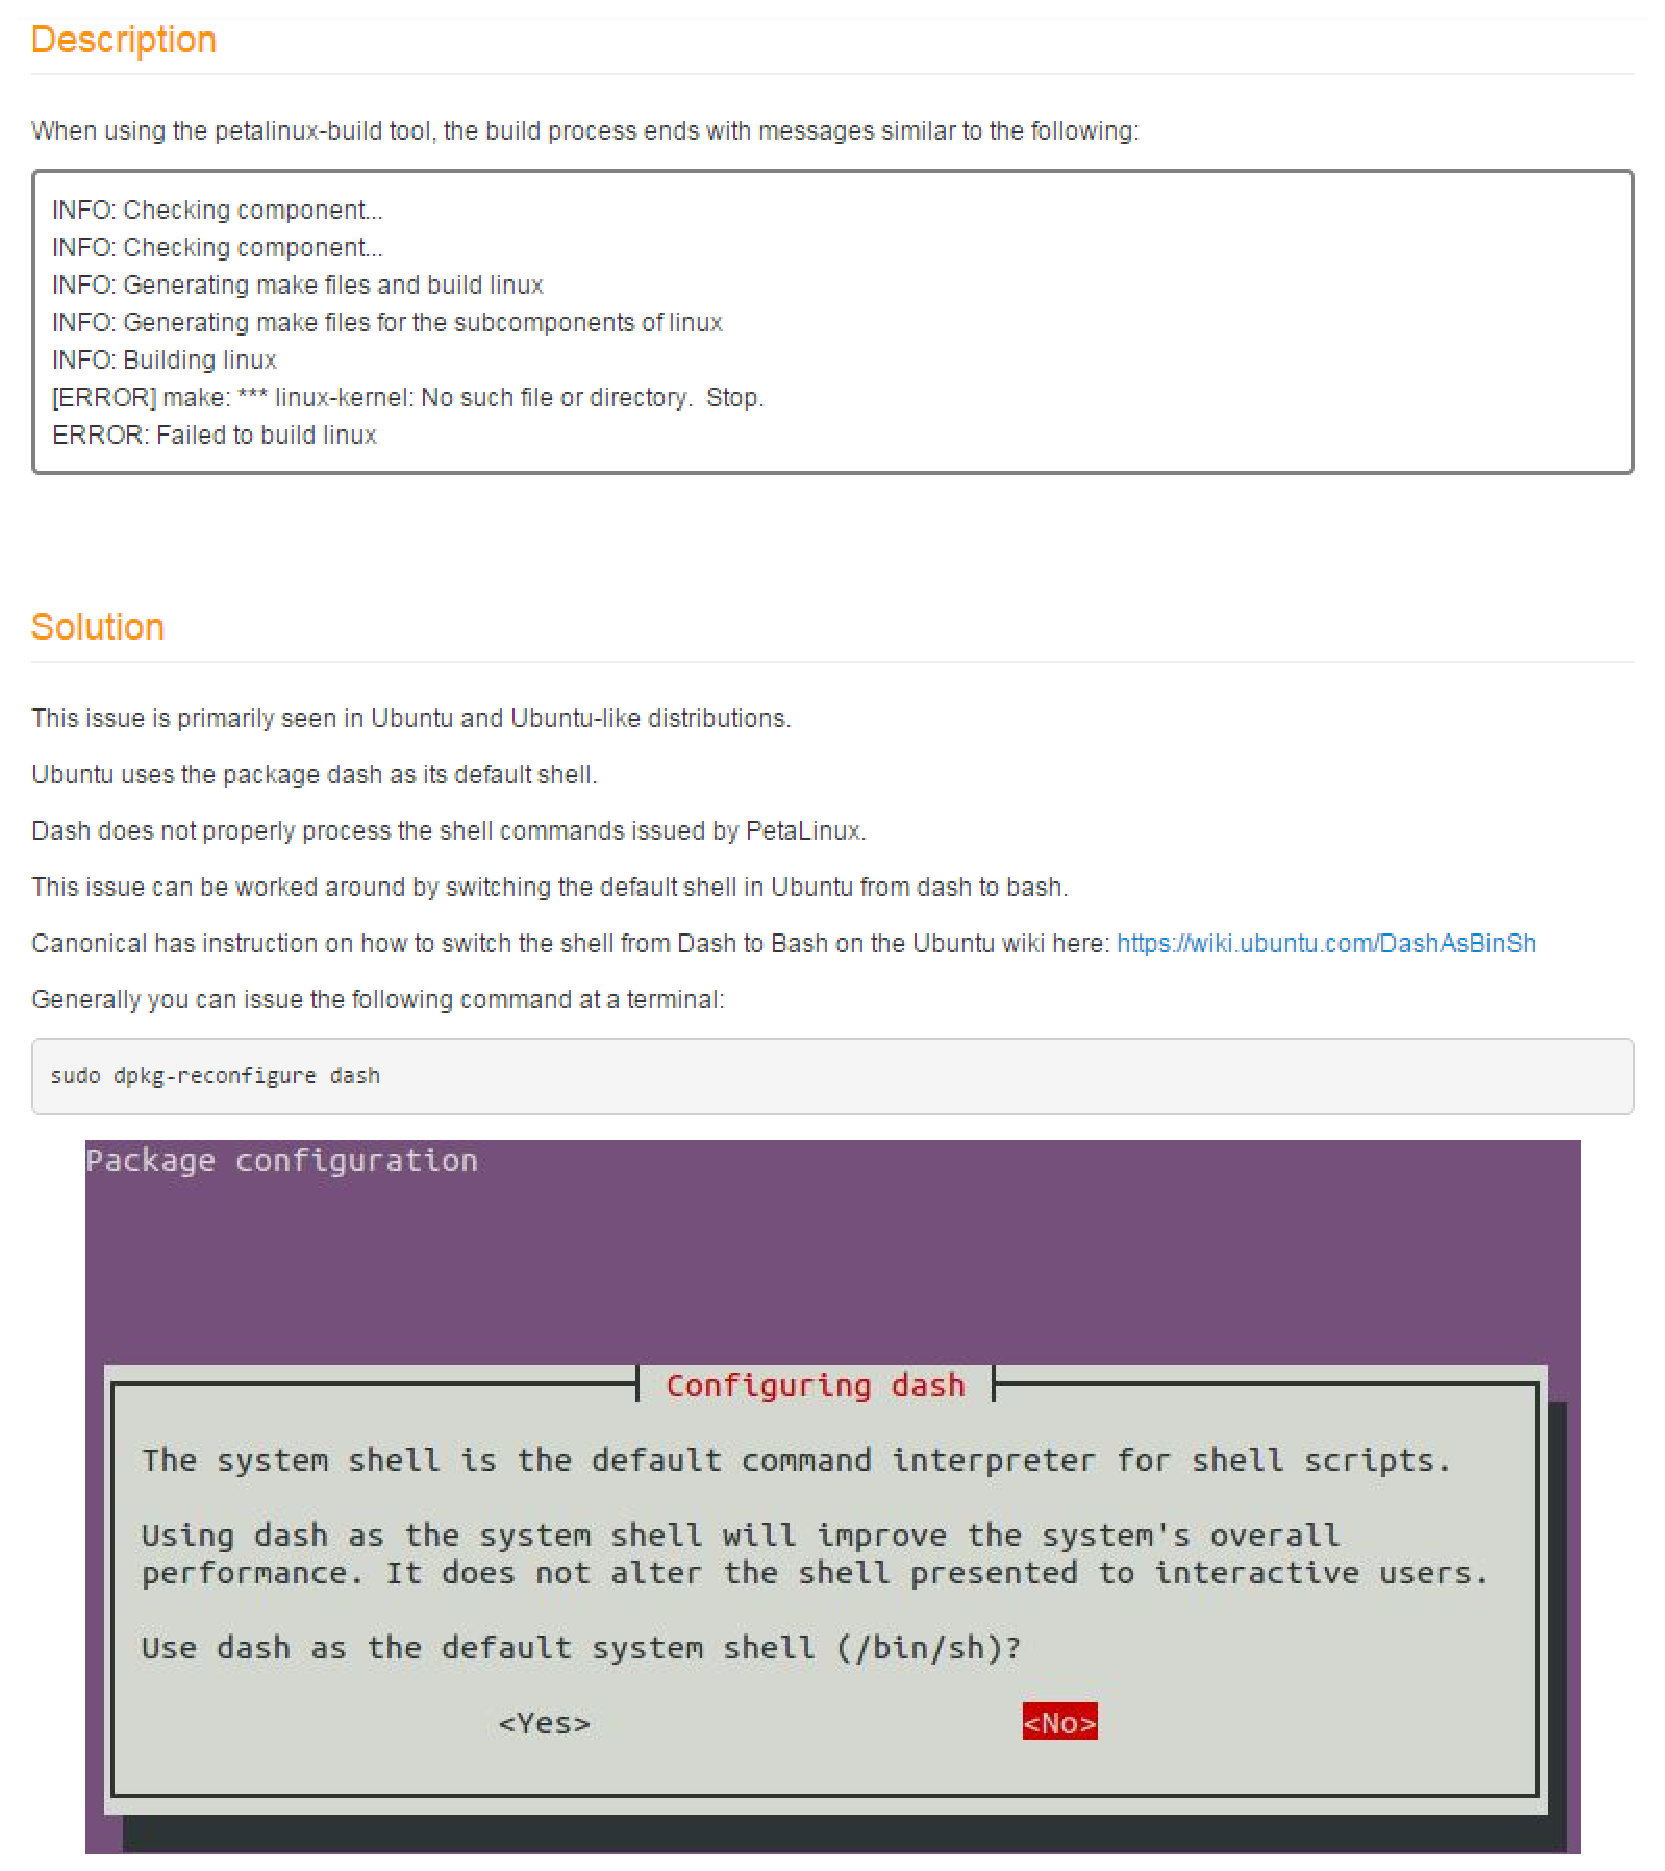
\includegraphics[width=0.85\textwidth]{./images/petalinux-build_error_solve.eps}
	\caption{Build Error}
	\label{fig:build_error} 
\end{figure}

재빌드시 아래와 같은 error 나는 상황이 발생하면 이는 처음 petalinux 설치전 설치하였던 패키지 중 libselinux1에 대한 모듈이 32bit용 모듈이 없기 때문이다.

\begin{lstlisting}[style=termstyle]
ctrluser@silee:~/Petalinux/training/buildBootImage/Avnet-Digilent-ZedBoard-2014.4$ petalinux-build 
INFO: Checking component...
INFO: Generating make files and build linux
INFO: Generating make files for the subcomponents of linux
INFO: Building linux
[INFO ] pre-build linux/rootfs/fwupgrade
[INFO ] pre-build linux/rootfs/peekpoke
[INFO ] pre-build linux/rootfs/uWeb
[INFO ] build linux/kernel
[INFO ] update linux/u-boot source
[INFO ] generate linux/u-boot configuration files
[INFO ] build linux/u-boot
[INFO ] build zynq_fsbl
[INFO ] Expanding stagefs
[ERROR] E: Sub-process /opt/pkg/petalinux-v2014.4-final/tools/packagemanager/bin/dpkg returned an error code (127)
[ERROR] make[2]: *** [.pkg_stagefs] Error 255
[ERROR] make[1]: *** [sub_build_component_/none/packages-repo/single/plnx-repo] Error 2
ERROR: Failed to build linux
\end{lstlisting}

이 문제를 해결하기 위하여는 32bit에서 설치된 libselinux.so.1 라이브러리를 64bit가 설치된 /lib32에 복사를 해주어야 한다.
또는 아래에서 build된 library를 다운 받는다. 안정적인 사용을 위하여는 Debian-32bit 시스템에서 복사해 오기 권장한다.

\begin{lstlisting}[style=termstyle]
http://forums.xilinx.com/t5/Embedded-Linux/2014-2-Image-Build-Processes-Error/td-p/476862/page/3
\end{lstlisting}

\begin{lstlisting}[style=termstyle]
ctrluser@silee:~/Petalinux/training/buildBootImage/Avnet-Digilent-ZedBoard-2014.4$ petalinux-build 
INFO: Checking component...
INFO: Generating make files and build linux
INFO: Generating make files for the subcomponents of linux
INFO: Building linux
[INFO ] pre-build linux/rootfs/fwupgrade
[INFO ] pre-build linux/rootfs/peekpoke
[INFO ] pre-build linux/rootfs/uWeb
[INFO ] build linux/kernel
[INFO ] update linux/u-boot source
[INFO ] generate linux/u-boot configuration files
[INFO ] build linux/u-boot
[INFO ] build zynq_fsbl
[INFO ] build linux/rootfs/fwupgrade
[INFO ] build linux/rootfs/peekpoke
[INFO ] build linux/rootfs/uWeb
[INFO ] build kernel in-tree modules
[INFO ] modules linux/kernel
[INFO ] post-build linux/rootfs/fwupgrade
[INFO ] post-build linux/rootfs/peekpoke
[INFO ] post-build linux/rootfs/uWeb
[INFO ] pre-install linux/rootfs/fwupgrade
[INFO ] pre-install linux/rootfs/peekpoke
[INFO ] pre-install linux/rootfs/uWeb
[INFO ] install system.dtb
[INFO ] install linux/kernel
[INFO ] update linux/u-boot source
[INFO ] generate linux/u-boot configuration files
[INFO ] build linux/u-boot
[INFO ] install linux/u-boot
[INFO ] install sys_init
[INFO ] install linux/rootfs/fwupgrade
[INFO ] install linux/rootfs/peekpoke
[INFO ] install linux/rootfs/uWeb
[INFO ] install kernel in-tree modules
[INFO ] modules_install linux/kernel
[INFO ] post-install linux/rootfs/fwupgrade
[INFO ] post-install linux/rootfs/peekpoke
[INFO ] post-install linux/rootfs/uWeb
[INFO ] package rootfs.cpio to /home/ctrluser/Petalinux/training/buildBootImage/Avnet-Digilent-ZedBoard-2014.4/images/linux
[INFO ] Update and install vmlinux image
[INFO ] vmlinux linux/kernel
[INFO ] install linux/kernel
[INFO ] package zImage
[INFO ] zImage linux/kernel
[INFO ] install linux/kernel
\end{lstlisting}

무사히 빌드가 완료 되었으면 아래 경로에 해당 linux 이미지가 생성됨을 확인한다. 해당 이미지를 확인 할 수 있다면 petalinux 툴 구성이 완료됨을 말한다.

\begin{lstlisting}[style=termstyle]
ctrluser@silee:~/Petalinux/training/buildBootImage/Avnet-Digilent-ZedBoard-2014.4/images/linux$ ls
image.elf  rootfs.cpio     system.dtb        u-boot.bin  u-boot-s.bin  u-boot.srec    urootfs.cpio.gz  zImage
image.ub   rootfs.cpio.gz  System.map.linux  u-boot.elf  u-boot-s.elf  u-boot-s.srec  vmlinux          zynq_fsbl.elf
\end{lstlisting}

\hfil\break

\chapter{DTC: Device Tree Compiler}


\section{구성}
Device Tree Compiler 구성은 아래 내용을 따른다.
\begin{lstlisting}[style=termstyle]
## Device Tree Copiler Tool
ctrluser@silee# aptitude install flex bison

## Device Tree Source Download
ctrluser@silee$git clone git://git.kernel.org/pub/scm/utils/dtc/dtc.git
ctrluser@silee$cd dtc;make
\end{lstlisting}
\section{Device Tree 작성}
The Device Tree is a data structure for describing hardware. Rather than hard coding every detail of a device into an operating system, many aspect of the hardware can be described in a data structure that is passed to the operating system at boot time. The device tree is used both by Open Firmware, and in the standalone Flattened Device Tree (FDT) form.
See the Device Tree Usage page for more details.
The data structure itself is a simple tree of named nodes and properties. Nodes contain properties and child nodes. Properties are simple name-value pairs. The structure can hold any kind of data.
However, in order to be useful, device tree data must be laid out in a structure that operating systems can understand. A "bindings" is a description of how a device is described in the device tree. Bindings for a lot of devices are well established and documented. You can read about them in the existing ePAPR and IEEE 1275 (OpenFirmware) documentation.
This site documents bindings not covered by either the ePAPR or IEEE 1275 specifications. If you need to describe a new device in the device tree, then you should document your binding on this site.

\chapter{U-Boot}
시스템을 처음 동작시키기 위해서는 시스템을 구동시켜 주는 부트로더가 필요하다. 이 부트로더는 시스템을 구동시킨 후 운영체제를 메모리에 로딩해 운영체제가 동작할 수 있도록 만들어 준다.  임베디드 시스템에서도 마찬가지이다. 시스템을 처음 동작시키기 위해서는 시스템을 구동시켜 주는 부트로더가 필요하다. 시스템의 전원을 켜면 ROM이나 FLASH 또는 하드디스크와 같은 저장장치에 있는 부트로더가 가장 먼저 실행되고, 이 부트로더는 시스템을 구동시킨 후 운영체제를 메모리에 로딩해 운영체제가 동작할 수 있도록 만들어 준다.부트로더는 기능이 간단하고 크기가 작은 프로그램이긴 하지만, 하드웨어 의존성이 강해 하드웨어의 구조를 이해해야만 작성할 수 있다. 그래서 보통은 보드 제작업체에서 하드웨어와 함께 탑재해 출시하는데, 간단한 구조이기 때문에 사용자가 직접 작성하기도 하고, 공개된 부트로더를 해당 보드에 맞게 고쳐서 사용하기도 한다. 공개된 부트로더를 이용하는 방식이 훨씬 만들기도 쉽고, 시리얼, 네트워크 등 여러 가지 기능을 이용할 수 있기 때문에 많이 사용되고 있다. 부트로더의 종류로는 U-boot, Blob, PMON, LILO, GRUB 등이 있고, 이중에서 임베디드 시스템에서 가장 많이 사용되는 것은 U-boot 이다. 타겟마다 사용되는 부트로더가 다르겠지만, 여기서는 가장 많이 사용되는 U-boot을 기준으로 진행하기로 한다.
\section{구성}
U-Boot 구성에 앞서 관련한 Tool에 대한 package를 설치한다.
\begin{lstlisting}[style=termstyle]
## conversion cross compiled vmlinux to u-boot image
ctrluser@silee# aptitude install u-boot-tools

## download u-boot source code, ftp://ftp.denx.de/pub/u-boot/

## cross compile 
ctrluser@silee$vi Makefile
# set default to nothing for native builds 
#ifeq ($(HOSTARCH),$(ARCH)) 
CROSS_COMPILE ?=arm-linux-gnueabihf- 
#endif
\end{lstlisting}
위와 같이 u-boot 의 컴파일 환경이 설정이 되었다면, 해당 CPU 아키텍쳐에 맞는 make 환경을 구성하여야 한다.
u-boot가 지원하는 CPU 아키텍쳐는 configs/xxx\_defconfig 로 명명되어 있다. 해당 u-boot 버전에서 지원하는 아키텍쳐의 리스트는 아래와 같다.

\begin{lstlisting}[style=termstyle]
...
mt_ventoux_defconfig                            zynq_microzed_defconfig
munices_defconfig                               zynq_zc70x_defconfig
mv88f6281gtw_ge_defconfig                       zynq_zc770_xm010_defconfig
mx23evk_defconfig                               zynq_zc770_xm012_defconfig
mx23_olinuxino_defconfig                        zynq_zc770_xm013_defconfig
mx25pdk_defconfig                               zynq_zed_defconfig
mx28evk_auart_console_defconfig                 zynq_zybo_defconfig
\end{lstlisting}

이중 우리가 타겟으로 삼는 ZedBoard(zynq\_zed\_defconfig)와 ZC706(zynq\_zc70x\_defconfig) 보드에 대한 config를 구성한다.

\begin{lstlisting}[style=termstyle]
#remove .config
ctrluser@silee$make mrproper

#make new .config
ctrluser@silee$make zynq_zed_config
ctrluser@silee$make

\end{lstlisting}

무사히 빌드가 성공되면 u-boot.bin이 생성된다. 이는 Zedboard Zynq의 FSBL(First Stage BootLoader)의 실행 후 Second Stage Boot로 실행 될 이미지이다. FSBL은 Vivado 툴에서 생성가능하다.

Analog Device에서 제공하는 각 보드별 Zynq의 ADC/DAC 보드를 보면 microSD 카드가 제공 되는데 이 카드를 보면 BOOT(FAT32) 영역과 rootfs(ext3) 영역으로 나뉘어지는데, BOOT 영역에는 각 CPU 보드별 BOOT.BIN이 들어 있다. BOOT.BIN의 구성은 FSBL.elf, u-boot.elf, bitstream 파일로 구성된다.


\chapter{Zynq구성}
\section{특성}

\begin{figure}[h!]
	\centering
	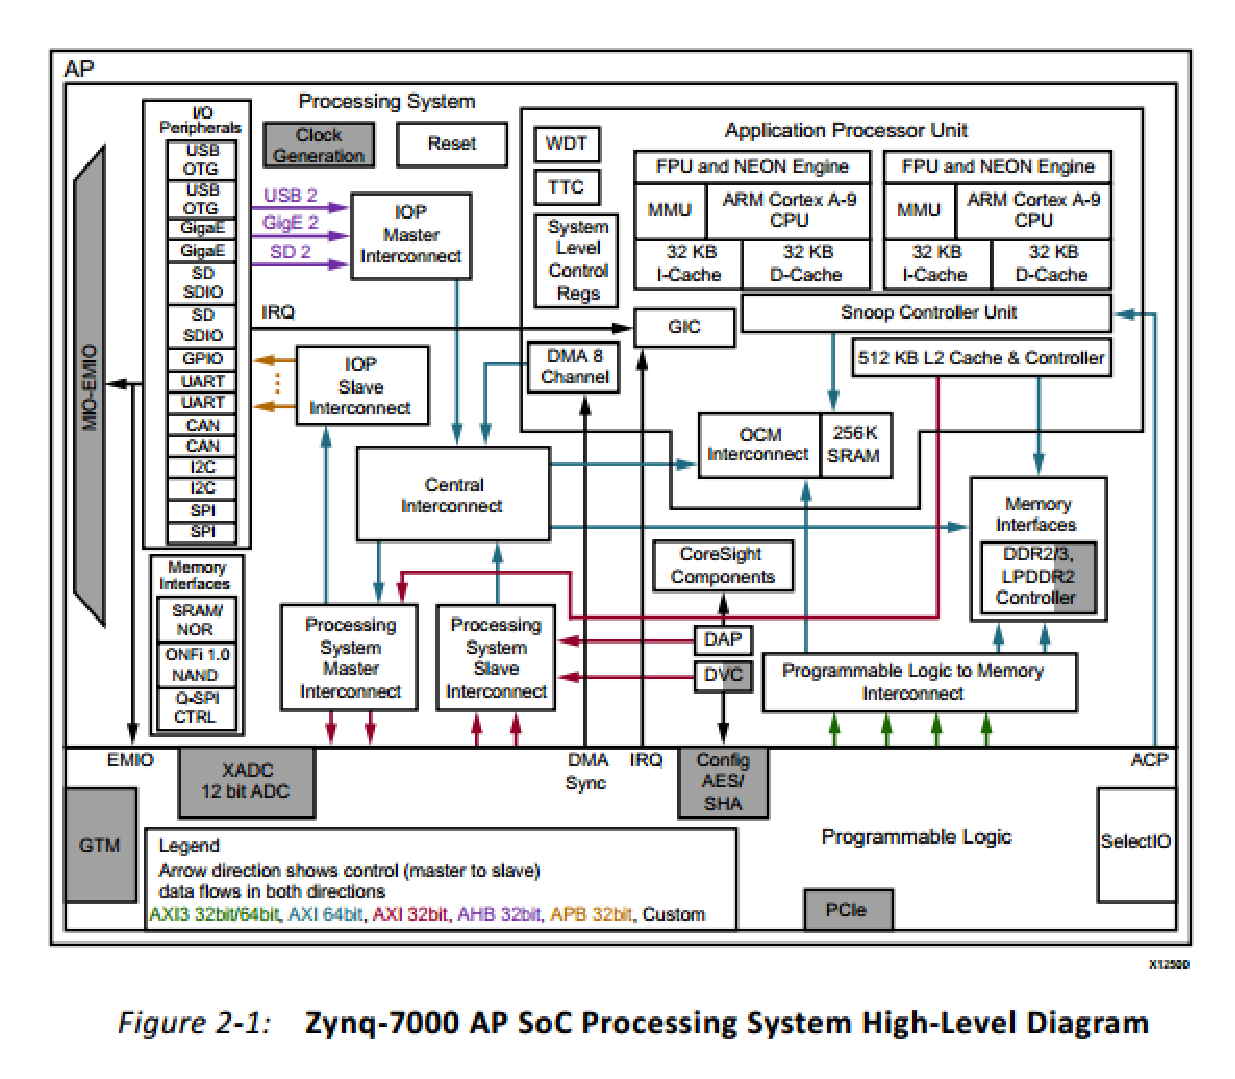
\includegraphics[width=0.95\textwidth, height=0.8\textwidth]{./images/zynq_arch.eps}
	\caption{Zynq Architecture}
	\label{fig:zynq_arch} 
\end{figure}


\section{Zynq Board Booting 방식}
요즘나오는 MCU 들은 다양한 부팅디바이스를 지원해야 한다.
MMC(SD)카드, NOR-Flash, NAND-Flash 등등...
이런 이유들로 MCU 내부에 아예 BootRom 이라는 코드가 내장되어 있다.
BootRom 은 플래시이며 이것이 실행될 당연하지만 RAM 영역도 있다.
Zynq 7000 시리즈 (ZC702, ZC706 내가 알고있고 사용한 zynq이다) 에는 내부 ROM 128K, 내부 SRAM 256K 가 있다.
파워리셋시 SRAM 주소는 0 번지이다.
파워리셋시 실행되는 코드를 Zynq에서는 BootRom 이라 명명한다.

BootRom이 시작되면 기본적인 PLL 설정등을 실행하고 부트디바이스를 검색한다.
부트디바이스는 MIO 라고 명명된 GPIO의 상태(H,L)를 보고 결정한다.
아래는 EV 보드 의 부팅스위치 사진이다
\begin{figure}[h!]
	\centering
	
\includegraphics[width=0.7\textwidth, height=0.7\textwidth]{./images/zynq_board.eps}
	\caption{Zynq Board}
	\label{fig:zynq_board} 
\end{figure}
만일 MMC 부팅이라면 MMC 디바이스에서 boot.bin 을 검색하여 이 파일을 메모리에 로드하고 이곳으로 점프한다.
NOR-Flash 나 QSPI-Flash 일 경우 0번지 부터 검색하여 특정값(FSBL-Header)이 있다면 데이타를 메모리에 로드한다.
NAND-Flash 의 경우 특정 페이지만큼 로드하겠지..(이건 데이타쉬트 안봄)

언급된 디바이스에서 최초 로드되는 것은 FSBL (FirstBootLoader) 이라고 하는 프로그램이다.
FSBL 은 자이링스가 제공하는 SDK에서 자동으로 생성하여 주는 코드이며 수정이 가능한다.
FSBL 에서는 DRAM 초기화, PLL 설정 등 필요한 하드웨어등을 설정한 후 주 부트로더를 메모리에 로드하고 점프한다.
일반적인 MCU 의 경우 소위 main.c 의 main()함수로 가기위해 start.S 라는 어셈블러코드와 작은 C 코드를 
따로 컴파일하고 이를 dd 유틸로 붙이는 작업을 하는데 이것을 제공되는 툴인 SDK 에서 제공하는 것이다.

FSBL을 컴파일 하여 만들어진 fsbl.elf 파일과 부트로더 즉 uboot.elf 파일을 합성하여 최종 boot.bin 이 만들어 진다.
이 합성툴의 이름은 bootgen.exe 이며 SDK 에서는 GUI 로 제공된다.

Zynq의 경우 FPGA 가 붙어있는 MCU 다 보니 따로 FPGA Bit 코드를 다운로드하여 주어야 한다.
FPGA를 구동할 코드는 VHDL, Veilog 등의 언어로 작성하고 ISE 툴을 사용하여 컴파일 한후 최종 .bit 파일 위에서 
소개된 bootgen 툴을 사용하여  세개의 파일 FSBL, uboot, fpga-bit 을 합성한다.
bit 파일이 포함되면 FSBL 코드에서 이를 다운로드한다.
bit 파일이 없을경우 다운로드 하지 않는다.
bit 파일은 uboot 에서나 이 후 커널부팅 후 다운로드 할수 있다.

Zynq 메뉴얼 ug585\_xxxxx.pdf 를 보면 부팅에 관련된 아주 상세한 내용을 찾을 수 있다.
Zynq 메뉴얼 ug873\_xxxxx.pdf 를 보면 SDK 등의 툴 사용법이 잘 기술되어 있다.

\section{Zynq Configuration}
ZYNQ는 보통 PS와 PL을 구분하여 이야기를 많이 합니다. PS는 기존 arm core가 들어간 SOC 영역을 의미하고, PL은 FPGA 영역을 의미합니다. ZYNQ는 기존 FPGA와는 다르게 PS 영역이 살아나야지만 정상 부팅을 하게 됩니다.FPGA만 따로 부팅할 수 없다는 이야기 입니다. 반대로 PL은 전혀 사용하지 않고 부팅은 가능 합니다. 하나씩 해보도록 하겠습니다.VIVADO 프로젝트를 만들고 Block Design을 만들어 줍니다. ZYNQ7 Processing System 을 추가해 주고 마우스로 더블클릭해 줍니다. 그러면 다음과 같이 IP를 설정하는 화면이 나오게 됩니다. 실제로 IP를 설정하기위해서는 Page Navigator에 있는 항목 전부 설정해줘야만 합니다. Xilinx에서 공식적으로 판매중인 장비에 대해서는 미리 설정된 파일이 있습니다. 표시한 Presets 을 선택해주면 제공하고 있는 장비가 나와 있습니다.여기서 사용중인 테스트 장비를 선택해주면 기본 설정이 완료됩니다. 저는 ZC706을 사용하기 때문에 ZC706로 선택 하였습니다. 상세한 설정이 궁금하신분은 Xilinx 홈페이지에서 ug898 문서를 확인하시길 바랍니다. 설정을 완료한 IP의 모습입니다. 설정에 따라 나와있는 핀들이 다를 수 있습니다.

\begin{figure}[h!]
	\centering
	\includegraphics[width=0.8\textwidth, height=0.8\textwidth]{./images/zynq_ps.eps}
	\caption{Zynq Processing System}
	\label{fig:zynq_ps} 
\end{figure}

ZYNQ가 부팅을 하기위해서는 최소한의 핀 설정이 필요합니다. VIVADO에서는 자동으로 설정해주는 기능을 제공하고 있습니다.
표시한 Run Block Automation 을 선택 해주면 다음과 같이 DDR과 FIXED\_IO가 나오게 됩니다. 

\begin{figure}[h!]
	\centering
	\includegraphics[width=0.8\textwidth, height=0.8\textwidth]{./images/zynq_ps_1.eps}
	\caption{Zynq Processing System - 1}
	\label{fig:zynq_ps_1} 
\end{figure}

위와같이 PS 관련 설정만 완료하면 ZYNQ는 부팅이 가능합니다. Create HDL Wrapper -> Run Synthesis -> Run Implementation -> Generate Bitstream 위 순서대로 진행을 하면 VIVADO에서 작업이 끝납니다.
다음 시간에는 부팅 이미지를 만들기 위해 u-boot와 kernel 이미지를 만들어 보겠습니다.

\begin{figure}[h!]
	\centering
	\includegraphics[width=0.8\textwidth, height=0.8\textwidth]{./images/zynq_ps_2.eps}
	\caption{Zynq Processing System-2}
	\label{fig:zynq_ps_2} 
\end{figure}

\section{Zynq Cross Compiler 설치}
u-boot나 kernel 모두 ARM에서 동작을 하기 때문에 build를 하기위해서는 cross compiler가 필요합니다. cross compiler를 설치하기 위해서는 방법이 여러가지 있습니다. 대표적으로 Xilinx에서는 peralinux 라는 개발환경을 제공하고 있습니다. 다른 방법으로는 cross compiler만 따로 설치하는 방법입니다.오늘은 cross compiler만 따로 설치해서 진행을 할 예정입니다.
아래 링크를 따라가면 cross compiler 설치 파일이 있습니다.

\begin{lstlisting}[style=termstyle]
https://code.google.com/p/zedboard-book-source/downloads/detail?name=xilinx-2011.09-50-arm-xilinx-linux-gnueabi.bin&can=2&q=xilinx-2011.09-50-arm-xilinx-linux-gnueabi.bin 
\end{lstlisting}
파일을 받으시면 됩니다.
설치 방법은 다음 링크를 보시면 쉽게 따라서 설치가 가능합니다.
\begin{lstlisting}[style=termstyle]
http://embedded.kleier.selfhost.me/xilinx_sourcery.php
\end{lstlisting}

!주의사항
ubuntu의 기본 쉘은 dash를 사용중입니다. 이 쉘을 bash로 변경해야만 설치가 가능합니다.
dash 를 bash로 변경하는 방법은 간단합니다.
\begin{lstlisting}[style=termstyle]
# sudo dpkg-reconfigure -plow dash
\end{lstlisting}
이후 NO 를 선택해 줍니다.

\begin{lstlisting}[style=termstyle]
# git clone https://github.com/Xilinx/u-boot-xlnx.git
# git clone https://github.com/Xilinx/linux-xlnx.git

# edit Makefile
# export ARCH=arm
# export CROSS_COMPILE=arm-xilinx-linux-gnueabi-
# export PATH=/opt/CodeSourcery/Sourcery_CodeBench_Lite_for_Xilinx_GNU_Linux/bin:$PATH

# arm-xilinx-linux-gnueabi-gcc --version
arm-xilinx-linux-gnueabi-gcc (Sourcery CodeBench Lite 2011.09-50) 4.6.1
Copyright (C) 2011 Free Software Foundation, Inc.
This is free software; see the source for copying conditions.  There is NO
warranty; not even for MERCHANTABILITY or FITNESS FOR A PARTICULAR PURPOSE.
\end{lstlisting}

!주의사항
64bit ubuntu를 사용중이라면 파일을 못찾는 경우가 생깁니다. 
이런경우 다음 페키지를 설치해야 합니다.
\begin{lstlisting}[style=termstyle]
# sudo apt-get install ia32-libs
\end{lstlisting}

설정이 완료되었으면 u-boot 부터 진행을 하겠습니다.
\begin{lstlisting}[style=termstyle]
# cd u-boot-xinx
\end{lstlisting}

파일 중 boards.cfg 라는 파일이 있습니다.이 파일에는 현재 u-boot가 지원하는 보드에 관하여 적혀있습니다.열어서 zynq를 검색해보면 다음과 같이 나옵니다. 디양한 설정이 있지만 자신에게 맞는 설정을 선택해야 합니다. 저는 ZC706보드를 사용중이기 때문에 zynq\_zc70x를 사용하겠습니다.

\begin{lstlisting}[style=termstyle]
# make zynq_zc70x_config
Configuring for zynq_zc70x board...

# make

# ls u-boot*
 u-boot* u-boot.bin u-boot.img u-boot.lds u-boot.map u-boot.srec
\end{lstlisting}

이많은 파일 중 우리가 필요한 파일은 u-boot 입니다. 다만 이름을 꼭 u-boot.elf로 변경 한 이후에 사용해야 합니다.그럼 다음으로 kernel 입니다.

\begin{lstlisting}[style=termstyle]
# cd ../linux-xlnx/
# ll arch/arm/configs/xilinx*
arch/arm/configs/xilinx_zynq_apf_defconfig
arch/arm/configs/xilinx_zynq_defconfig

# make xilinx_zynq_defconfig
HOSTCC  scripts/basic/fixdep
HOSTCC  scripts/kconfig/conf.o
SHIPPED scripts/kconfig/zconf.tab.c
SHIPPED scripts/kconfig/zconf.lex.c
SHIPPED scripts/kconfig/zconf.hash.c
HOSTCC  scripts/kconfig/zconf.tab.o
HOSTLD  scripts/kconfig/conf
#
# configuration written to .config
#
\end{lstlisting}

설정이 완료되면 다시 make를 통해 진행 합니다.

\begin{lstlisting}[style=termstyle]
# make UIMAGE_LOADADDR=0x8000 uImage

"mkimage" command not found - U-Boot images will not be built

# aptitude install u-boot-tools
# ls arch/arm/boot/
.Image.cmd .gitignore .uImage.cmd .zImage.cmd Image* Makefile install.sh uImage zImage*
\end{lstlisting}

kernel 이미지 파일은 3가지 종류로 나옵니다.Image, uImage, zImage 중 u-boot용인 uImage를 사용합니다. 여기까지가 부팅에 필요한 u-boot.elf와 uImage 만든는 방법이였습니다. ZYNQ를 부팅하기위해서는 중요한 마지막 작업이 남아있습니다.

\section{Zynq Boot.bin 만들기}

BOOT.bin 파일은 원래 부팅에 필요한 다른파일을 하나로 합친 파일입니다.보통 FSBL + Bitstream + user application(u-boot) 하나씩 살펴보면 Bitstream 은 VIVADO에서 Generate Bitstream을 통해 나온 파일입니다.(~~.bit) FSBL 은 First Stage Bootloader의 약자입니다. OCM 에서 동작을 시작해 시본적인 설정들을 초기화 해줍니다. DDR도 여기서 설정을 해줍니다.  그 후 Bitstream 가 있다면 FPGA 부분을 활성화 해줍니다. 마지막으로 user application을 DDR 메모리에 복사하여 구동시켜 줍니다.
매우 중요하고 복작해 보이죠? 다행이도 SDK에서 자동으로 생성해 줍니다.!!마지막으로 user application은 SDK에서 작성한 프로그램이나 U-boot.elf 를 뜻합니다.이 3개의 파일을 하나로 만들면 boot.bin 이 됩니다. 이것도 SDK에서 가능합니다. 그럼 SDK를 실행해보겠습니다.우선 전에 진행했던 VIVADO 프로젝트를 열어 줍니다. 그리고 Block Design을 열어줍니다. 그 후 다음 그림과 같이 Export Hardware 메뉴를 선택해 줍니다.

\begin{figure}[h!]
	\centering
	\includegraphics[width=0.95\textwidth]{./images/boot_bin.eps}
	\caption{Boot.bin}
	\label{fig:boot.bin} 
\end{figure}
다음과 같이 include bitstream을 선택해 줍니다.

\begin{figure}[h!]
	\centering
	
\includegraphics[width=0.7\textwidth]{./images/boot_bin_1.eps}
	\caption{Boot.bin-1}
	\label{fig:boot.bin.1} 
\end{figure}
IVADO 2014.1 이전 까지만 해도 이 메뉴에 Launch SDK 가 있었지만 2014.2 버전에는 따로 나와 있습니다. file -> Launch SDK 메뉴를 선택해 주면 SDK가 실행 됩니다. 설정은 디폴트로 하는것이 편합니다. 그리고 Block Design이 열려있지 않다면 SDK가 실행되지 않을 수 있습니다. SDK를 따로 실행해도 되지만 Block Design의 정보를 가져오기 위해서는 VIVADO를 통해서 실행하는것이 편합니다.
SDK는 요즘 많이 사용하는 eclipse 기반으로 만들어져 있습니다. 그러면 FSBL을 만들어 보겠습니다. File -> New -> Application Project 를 선택해 주세요. 프로젝트 이름은 zynq\_fsbl로 했습니다. 다른 설정은 필요없고 기존에 사용하던 BSP가 있다면 아래 그림처럼 선택해 주고 아니면 새로 생성해 줍니다.

\begin{figure}[h!]
	\centering
	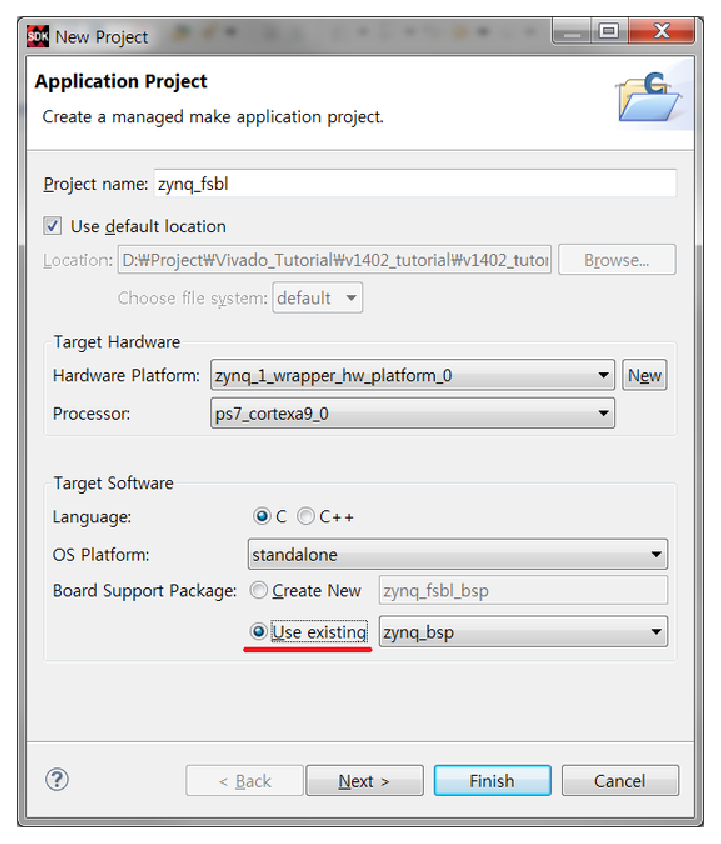
\includegraphics[width=0.8\textwidth]{./images/boot_bin_3.eps}
	\caption{Boot.bin-2}
	\label{fig:boot.bin.2} 
\end{figure}

\clearpage

Next를 눌러 주면 다음과 같이 기본 템플릿을 제공합니다. 이중 Zynq FSBL이 있습니다. 이걸 선택하소 Finish를 눌러주면 FSBL이 생성됩니다. 그러면 대충 필요한 파일들이 모였습니다. FSBL은 오늘 만들었고 Bitstream은 첫번째 시간에 만들었습니다.이것들을 가지고 BOOT.BIN 파일을 만들어 보겠습니다. SDK에서 다음 그림과 같이 Create Zynq Boot Image 를 선택해 줍니다.

\begin{figure}[h!]
	\centering
	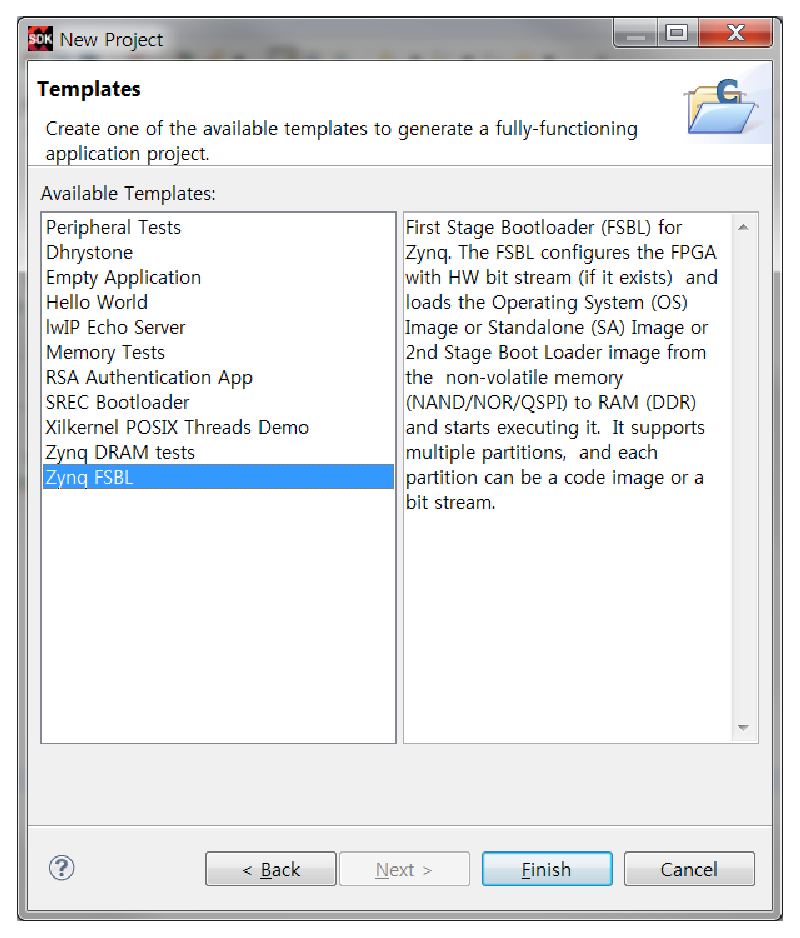
\includegraphics[width=0.8\textwidth]{./images/boot_bin_4.eps}
	\caption{Boot.bin-3}
	\label{fig:boot.bin.3} 
\end{figure}

실행하시면 다음과 같은 화면이 나옵니다.한번 boot.bin을 만들면 설정파일(BIF)을 저장하게 됩니다. 이 설정파일이 저장되는 우치를 적당한곳에 설정을 해줍니다.그리고 boot.bin에 들어갈 파일(FSBL.elf, bit파일, u-boot.elf)을 추가해야 합니다.

\begin{figure}[h!]
	\centering
	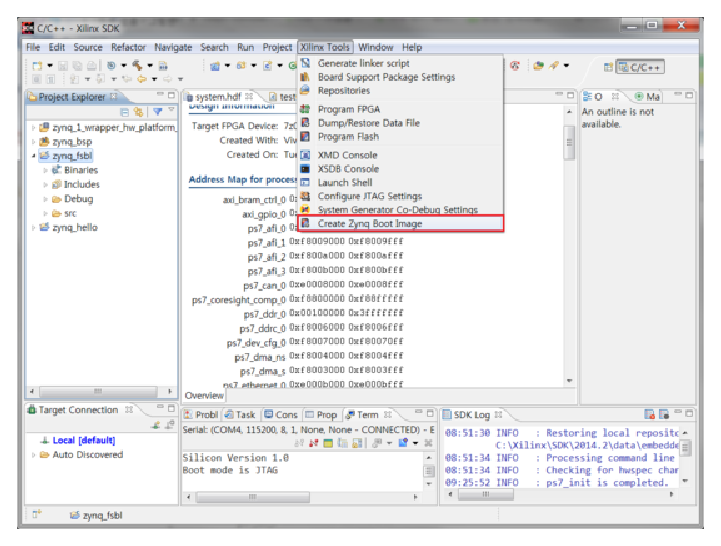
\includegraphics[width=0.95\textwidth]{./images/boot_bin_5.eps}
	\caption{Boot.bin-4}
	\label{fig:boot.bin.4} 
\end{figure}

add를 누른 화면입니다. 먼저 FSBL.elf를 추가해 줍니다.이때 FSBL은 type을 bootloader로 설정해 주어야 합니다.

\begin{figure}[h!]
	\centering
	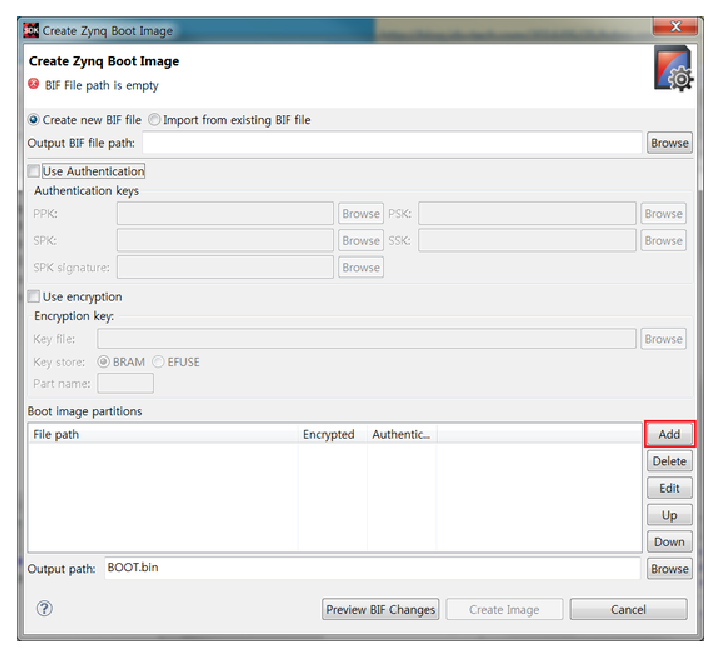
\includegraphics[width=0.95\textwidth]{./images/boot_bin_6.eps}
	\caption{Boot.bin-5}
	\label{fig:boot.bin.5} 
\end{figure}

다음은 bit파일을 추가해 주겠습니다.bit파일은 SDK를 실행할 때 같이 만들어지도록 설정을 해주었다면 hw\_platform 폴더에들어있습니다.
사용자 설정에 따라 폴더이름이 변경됩니다. 저는 zynq\_1\_wrapper\_hw\_platform\_0 폴더에 zynq\_1\_wrapper.bit라는 이름으로 생성되어 있었습니다.이번에는 type을 datafile로 설정해 줍니다.

\begin{figure}[h!]
	\centering
	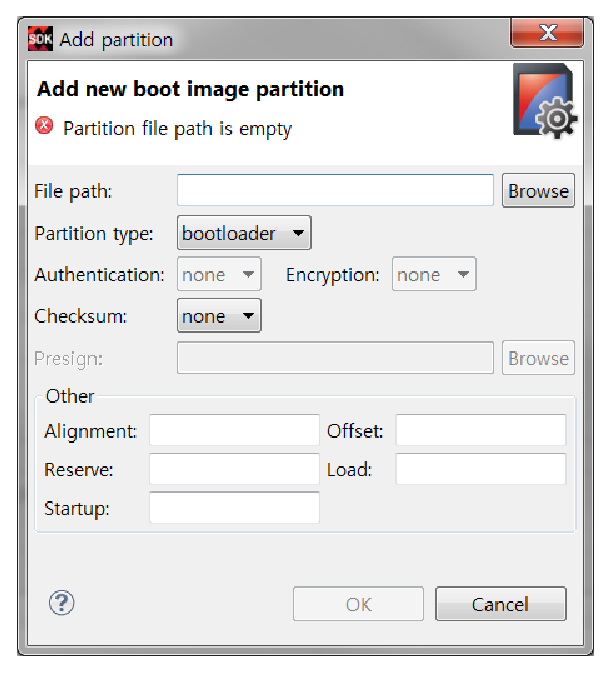
\includegraphics[width=0.95\textwidth]{./images/boot_bin_7.eps}
	\caption{Boot.bin-6}
	\label{fig:boot.bin.6} 
\end{figure}

\clearpage
\begin{figure}[h!]
	\centering
	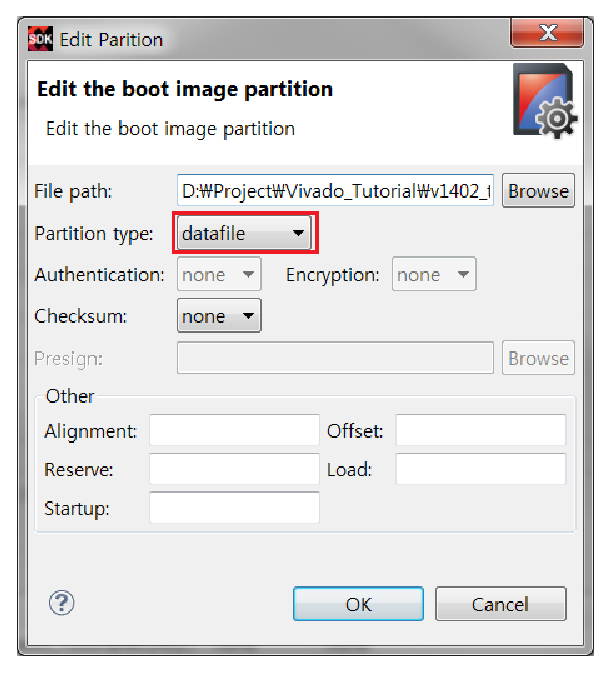
\includegraphics[width=0.95\textwidth]{./images/boot_bin_8.eps}
	\caption{Boot.bin-7}
	\label{fig:boot.bin.7} 
\end{figure}

마지막으로 오늘 맨 처음 Xilinx 에서 받은 파일 중 u-boot.elf파일을 추가해 줍니다.이 파일도 datafile 로 설정해 줍니다. 
필요한 파일으 추가한 모습입니다.아까 FSBL.elf만 설정이 다르기 때문에 나타나는 모습도 다른것을 볼 수 있습니다. Output path를 설정해 주시고 Create Image를 누르면 Output path에 설정되 경로에 생성됩니다.(경로에 파일명도 넣어주셔야 합니다.)
\begin{figure}[h!]
	\centering
	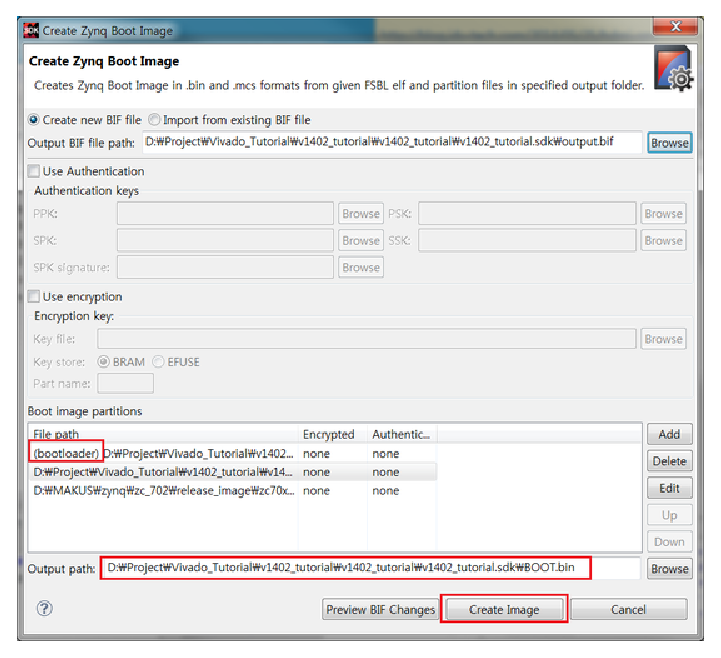
\includegraphics[width=0.95\textwidth]{./images/boot_bin_9.eps}
	\caption{Boot.bin-8}
	\label{fig:boot.bin.8} 
\end{figure}


\clearpage

\bibliographystyle{unsrtnat}
\bibliography{./refs}

\end{document}

